\documentclass{../../slides-style}

\slidetitleext{Лекция 5: Управление проектом}{10.04.2025}{Управление проектом}

\begin{document}

    \begin{frame}[plain]
        \titlepage
    \end{frame}

    \section{Отслеживание}

    \begin{frame}
        \frametitle{Отслеживание прогресса проекта}
        \begin{itemize}
            \item Задачи
            \begin{itemize}
                \item Небольшой объём
                \item Чёткие критерии завершенности
                \item Регулярные обновления статуса
                \begin{itemize}
                    \item Правило 0-50-100
                \end{itemize}
            \end{itemize}
            \item Люди
            \begin{itemize}
                \item Регулярные (еженедельные) отчёты 
            \end{itemize}
            \item Дефекты
            \item Коммиты
            \item График
            \begin{itemize}
                \item Диаграмма Гантта
                \item Критический путь
                \item Измерение прогресса, а не затрат
            \end{itemize}
        \end{itemize}
    \end{frame}

    \begin{frame}{Метрики}
        \begin{itemize}
            \item Зачем: оценка соответствия плану, использования ресурсов, фактический материал для обсуждений
            \begin{itemize}
                \item Метрики полезны только если используются при обсуждениях и при принятии решений!
            \end{itemize}
            \item Что: опережающие и запаздывающие индикаторы
            \begin{itemize}
                \item Измерять \emph{дорого}: \enquote{SMART}-метрики
                \item Типовые метрики: 
                \begin{itemize}
                    \item Технические по уже задеплоенному приложению
                    \item Метрики хода разработки
                    \item Метрики стоимости и графика
                    \item Метрики использования ресурсов
                    \item Бизнес-метрики
                    \item Удовлетворённость ключевых участников
                    \item Прогнозные метрики
                \end{itemize}
            \end{itemize}
        \end{itemize}
    \end{frame}

    \begin{frame}{Метрики хода разработки}
        \begin{itemize}
            \item Работа в процессе~--- сколько задач в статусе Doing
            \item Время выполнения задачи (Lead time)~--- время от попадания в бэклог (или взятия обязательств) до релиза
            \item Время цикла (Cycle time)~--- сколько из времени выполнения потрачено собственно на разработку
            \item Размер очереди~--- сколько задач в статусе To Do
            \item Размер \enquote{партии} (Batch size)~--- сколько работы делается за итерацию (Team Velocity в Scrum)
            \item Эффективность процесса~--- отношение времени, потраченного на полезную работу (создающую value), ко времени, потраченному на вспомогательные активности
        \end{itemize}
    \end{frame}

    \begin{frame}{Методика освоенного объёма (Earned Value)}
        \begin{itemize}
            \item Совокупная запланированная стоимость (Budget at completion, BAC)~--- общий бюджет проекта минус резерв
            \item Плановый объём (Planned value, PV, он же Budgeted cost of work scheduled, BCWS)~--- плановая стоимость запланированных на данный момент работ
            \item Освоенный объём (Earned value, EV, он же Budgeted cost of work performed, BCWP)~--- плановая стоимость реально выполненного на данный момент объёма работ ($EV = \text{процент завершения проекта} * BAC$)
            \item Фактическая стоимость (Actual cost, AC, она же Actual cost of work performed, ACWP)~--- фактическая стоимость реально выполненного на данный момент объёма работ
        \end{itemize}
    \end{frame}

    \begin{frame}{Производные метрики}
        \begin{itemize}
            \item Отклонение по стоимости (Cost variance, CV)~--- разница фактической и расчётной стоимости ($CV = EV - AC$)
            \item Отклонение по срокам (SV, Schedule variance)~--- запаздывание или опережение графика ($SV = EV - PV$)
            \item Индекс стоимости работ (Cost performance index, CPI)~--- показывает, насколько проект тратит деньги быстрее/медленнее ожидаемого ($CPI = EV / AC$)
            \item Индекс сроков выполнения (Schedule performance index, SPI)~--- показывает, насколько команда работает быстрее/медленнее ожидаемого ($SPI = EV / PV$)
        \end{itemize}
        CV и SV должны быть больше нуля, CPI и SPI больше 1
    \end{frame}

    \begin{frame}{Производные метрики}
        \begin{center}
            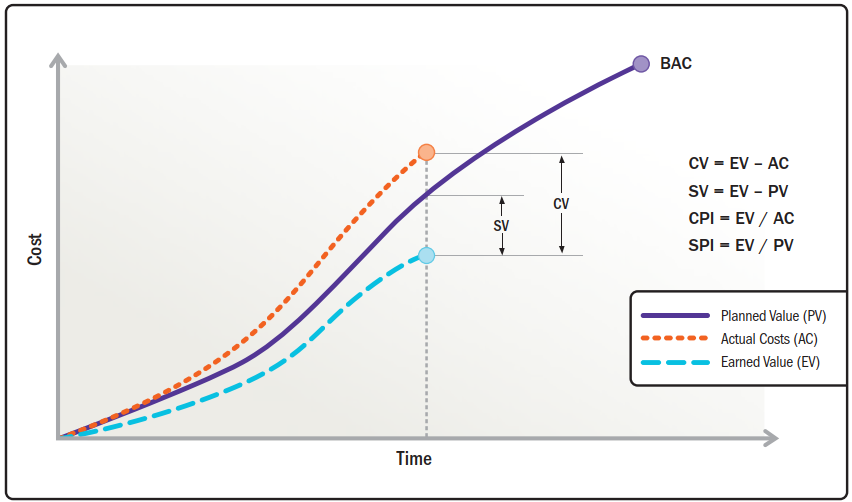
\includegraphics[width=0.9\textwidth]{svCvMetricsGraph.png}
            \attribution{PMBOK 7}
        \end{center}
    \end{frame}

    \begin{frame}{Прогнозные метрики}
        \begin{itemize}
            \item Прогноз для завершения (Estimate to complete, ETC) --- ожидаемая стоимость окончания всех оставшихся работ (обычно считается как $ETC = (BAC - EV) / CPI$)
            \item Прогноз по завершении (Estimate at completion, EAC) --- ожидаемая стоимость всех работ в целом (\enquote{настоящий} BAC)
            \item Отклонение при завершении (Variance at completion, VAC) --- прогноз разницы между фактическим и запланированным бюджетом ($VAC = EAC - BAC$)
            \item Индекс производительности до завершения (To-complete Performance Index, TCPI) --- показывает эффективность трат для достижения цели проекта ($TCPI =  ETC / (BAC - AC)$)
        \end{itemize}
    \end{frame}

    \begin{frame}{Прогнозные метрики}
        \begin{center}
            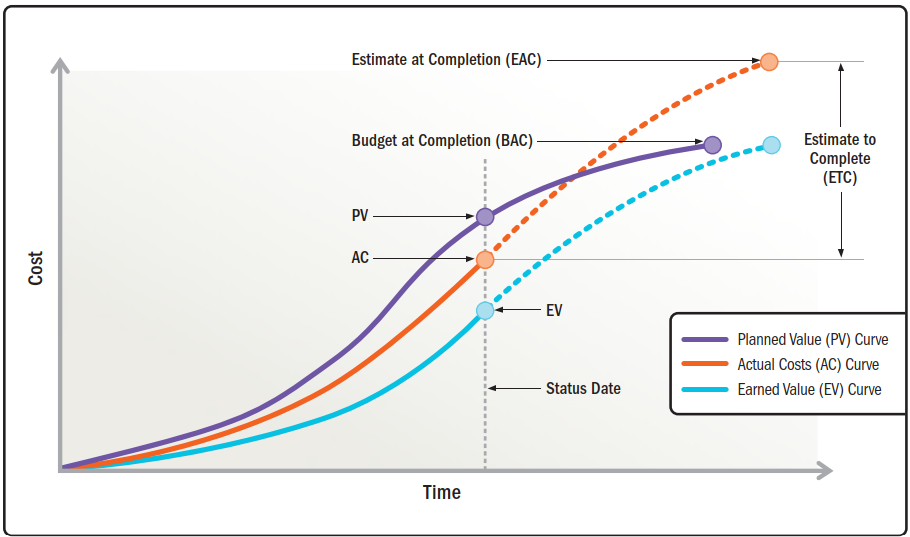
\includegraphics[width=0.9\textwidth]{eacEtcMetricsGraph.png}
            \attribution{PMBOK 7}
        \end{center}
    \end{frame}

    \begin{frame}{Бизнес-метрики}
        \begin{itemize}
            \item Соотношение затрат и выгод --- отношение ожидаемой ценности для бизнеса к стоимости проекта (может быть меньше 1, если есть законодательные, социальные или другие причины браться за проект)
            \item Запланированная ценность относительно актуальной ценности
            \item Возврат инвестиций (Return of investment, ROI) --- отношение текущей стоимости проекта к затратам (в деньгах)
            \item Чистая приведенная стоимость (Net Present Value, NPV) --- разница между инвестициями и прибылью (если она меньше нуля, то проект, скажем так, пока только подаёт надежды)
            \begin{itemize}
                \item Есть некоторые бухгалтерские тонкости, связанные с понятием \enquote{приведённая} (т.е. с учётом инфляции)
            \end{itemize}
        \end{itemize}
    \end{frame}

    \begin{frame}{Метрики заинтересованных сторон}
        \begin{itemize}
            \item Чистый балл промоутера (Net promoter score, NPS) --- балл от -100 до 100, показывающий, насколько пользователь готов рекомендовать продукт другим
            \item Диаграмма настроения --- отслеживает настроение команды
            \item Мораль команды
            \begin{itemize}
                \item \enquote{Я чувствую, что моя работа вносит свой вклад в достижение общих результатов}
                \item \enquote{Я чувствую, что меня ценят}
                \item \enquote{Я доволен тем, как моя проектная команда работает вместе}
            \end{itemize}
            \item Текучка кадров
        \end{itemize}
        \begin{center}
            
\includegraphics[width=0.6\textwidth]{moodChart.png}
            \attribution{PMBOK 7}
        \end{center}
    \end{frame}

    \begin{frame}
        \begin{center}
            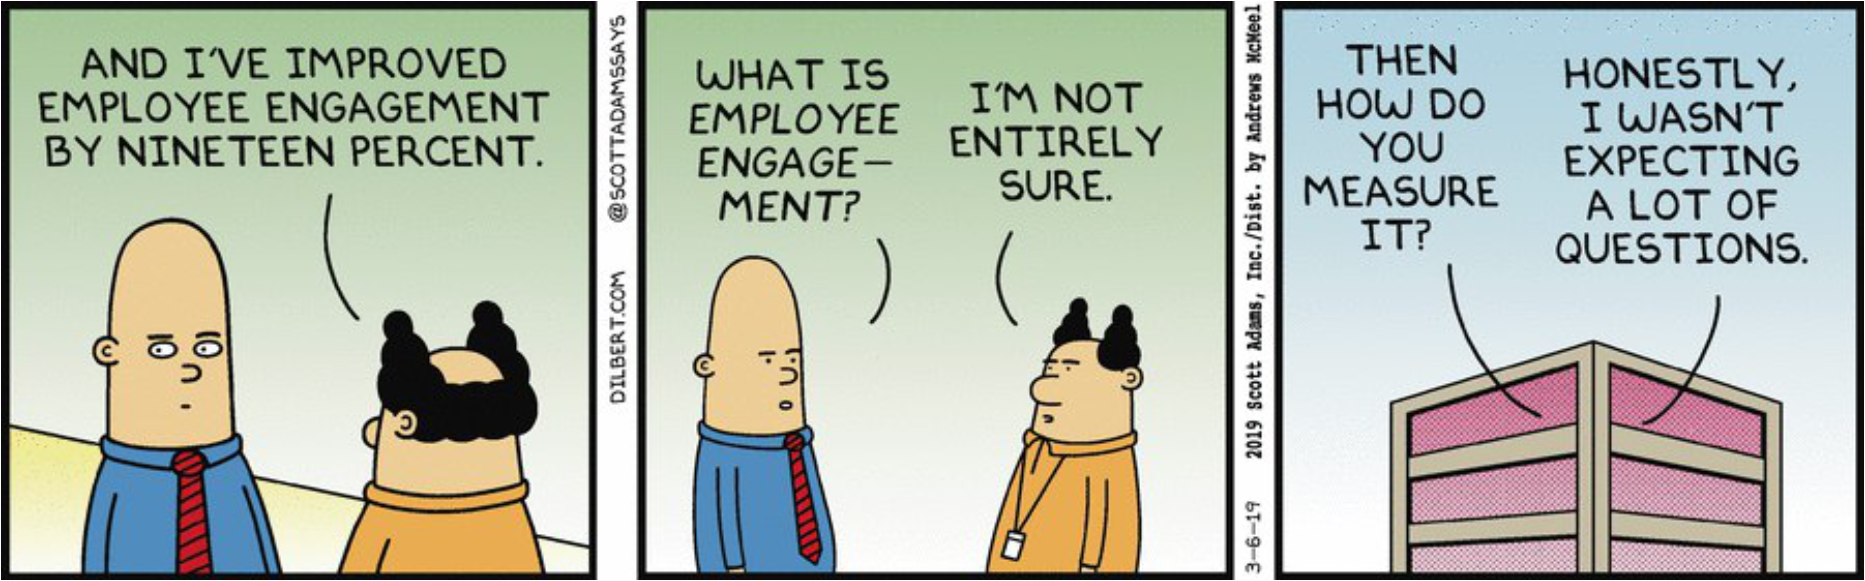
\includegraphics[width=0.9\textwidth]{dilbertEmployeeEngagement.png}
        \end{center}
    \end{frame}

    \begin{frame}
        \frametitle{Отслеживание затрат и времени}
        \begin{center}
            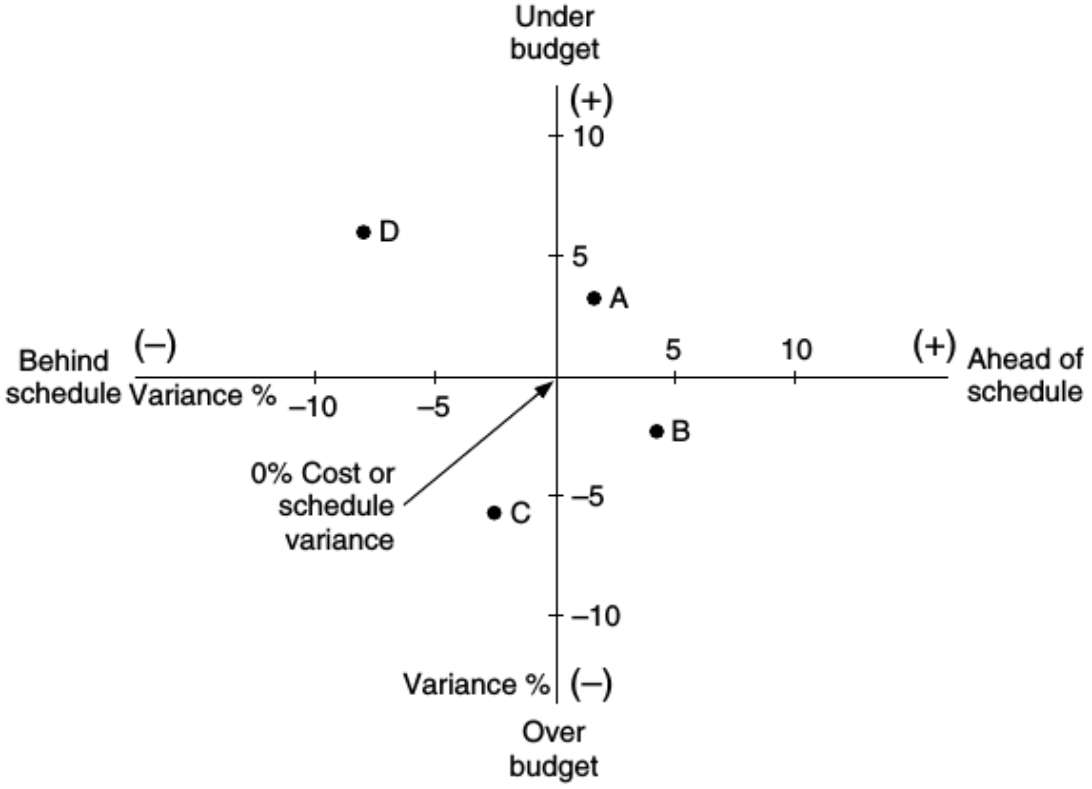
\includegraphics[width=0.8\textwidth]{varianceGraph.png}
        \end{center}
    \end{frame}

    \begin{frame}
        \frametitle{Пороги эскалации}
        \begin{center}
            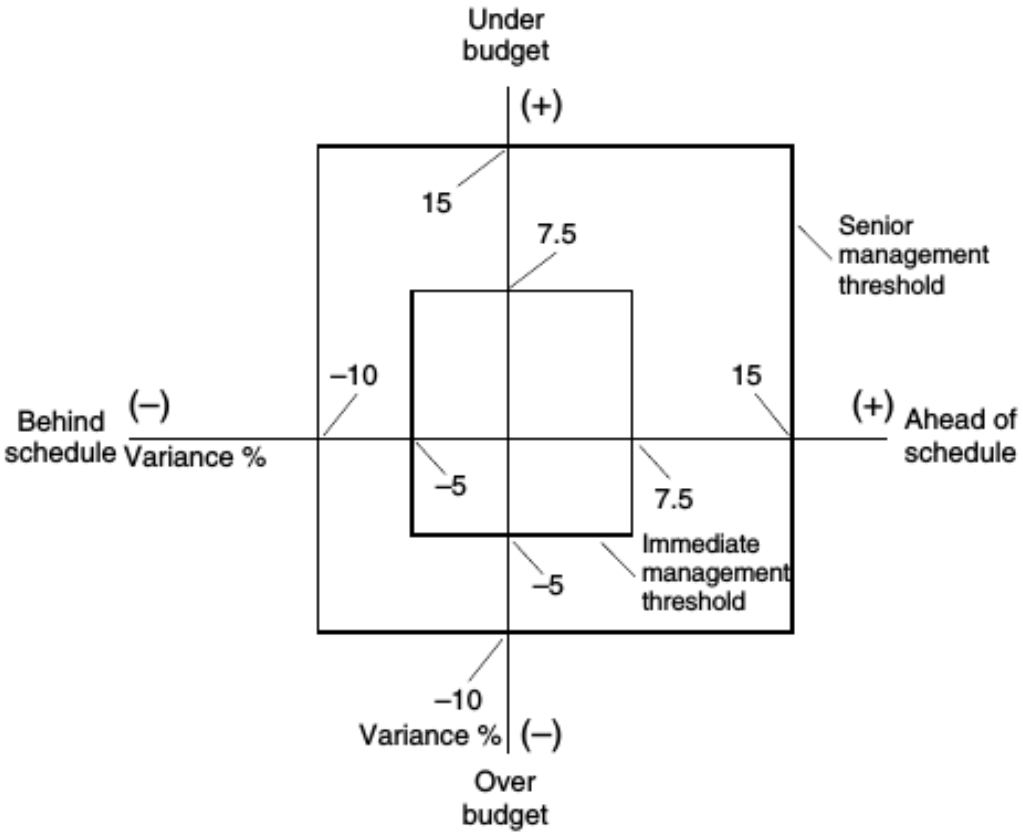
\includegraphics[width=0.7\textwidth]{escalationThresholds.png}
        \end{center}
    \end{frame}

    \begin{frame}{Трудности в измерении}
        \begin{itemize}
            \item Эффект Хоторна (Hawthorne effect) --- сам факт измерения меняет поведение измеряемой системы
            \item Пустые метрики
            \item Деморализация из-за недостижимых целевых показателей
            \item Неправильное использование метрик
            \begin{itemize}
                \item Фокусирование на неважных метриках
                \item Фокусирование на достижении кратковременных целевых показателях в ущерб долгосрочным
                \item \enquote{Достигательство}
            \end{itemize}
            \item Предвзятость подтверждения (Confirmation bias)
            \item Корреляция не влечёт причинность
        \end{itemize}
    \end{frame}

    \section{Балансирование}

    \begin{frame}
        \frametitle{Треугольник равновесия}
        \begin{columns}
            \begin{column}{0.5\textwidth}
                \begin{center}
                    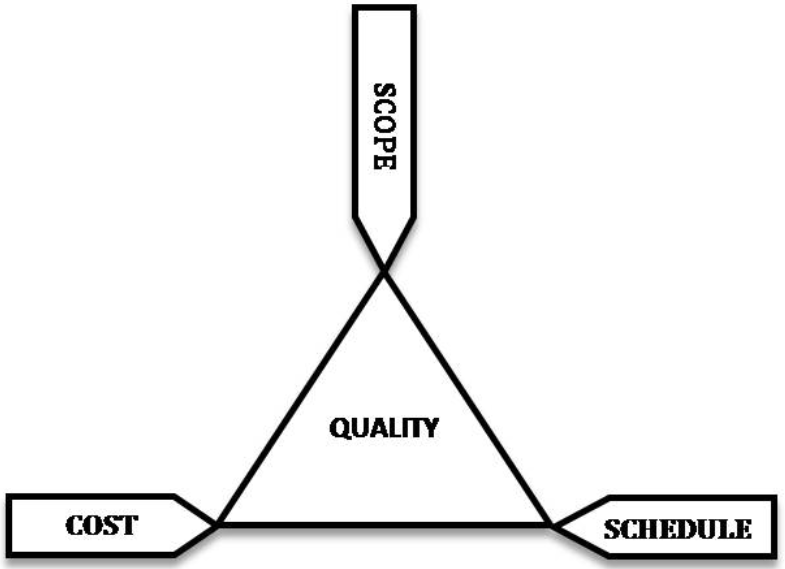
\includegraphics[width=0.9\textwidth]{balanceTriangle.png}
                \end{center}
            \end{column}
            \begin{column}{0.5\textwidth}
                \begin{center}
                    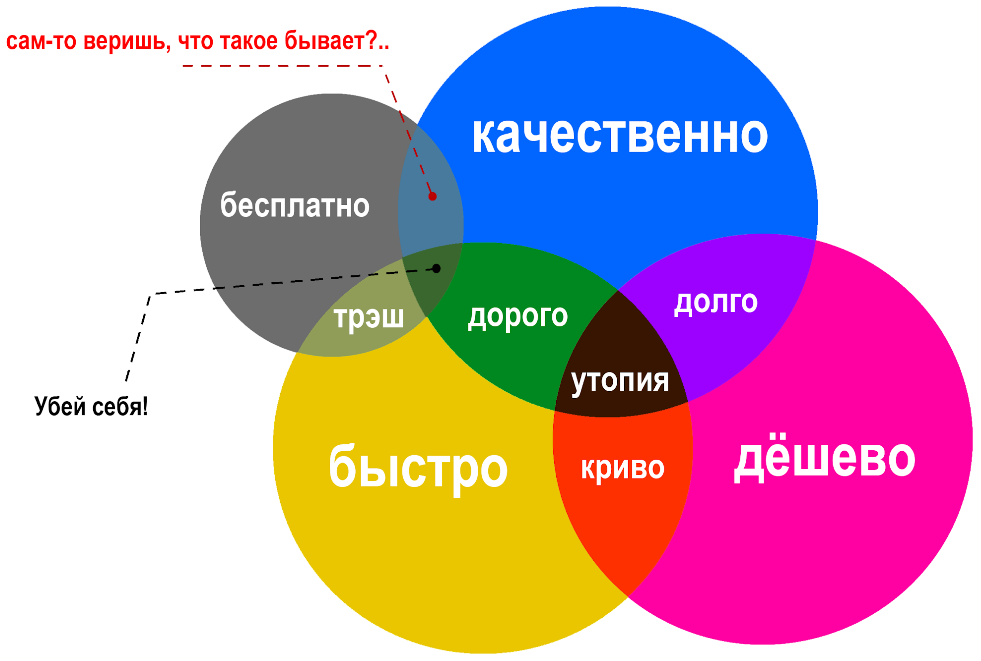
\includegraphics[width=0.9\textwidth]{balanceTriangleExplained.png}
                \end{center}
            \end{column}
        \end{columns}
    \end{frame}

    \begin{frame}
        \frametitle{Балансирование на уровне проекта}
        \begin{itemize}
            \item Повторная оценка задач
            \item Перераспределение задач критического пути
            \item Добавление людей в проект
            \item Привлечение экспертов
            \begin{itemize}
                \item Внутренние и внешние
                \item Создание экспертов внутри проекта
            \end{itemize}
            \item Аутсорсинг частей проекта
            \item Сверхурочная работа
            \item Снижение качества проекта
        \end{itemize}
    \end{frame}

    \begin{frame}
        \frametitle{Балансирование на уровне бизнес-целей}
        \begin{itemize}
            \item Изменение границ проекта
            \item Подстраивание проекта под дедлайны
            \item Работа на опережение
            \item Incremental delivery
            \item Создание прототипа
            \item Снижение прибыльности проекта
        \end{itemize}
    \end{frame}

\end{document}
